\documentclass{standalone}
\usepackage{tikz}
\usetikzlibrary{patterns, positioning}
\usepackage[sfdefault]{ClearSans} %% option 'sfdefault' activates Clear Sans as the default text font
\usepackage[T1]{fontenc}

\begin{document}
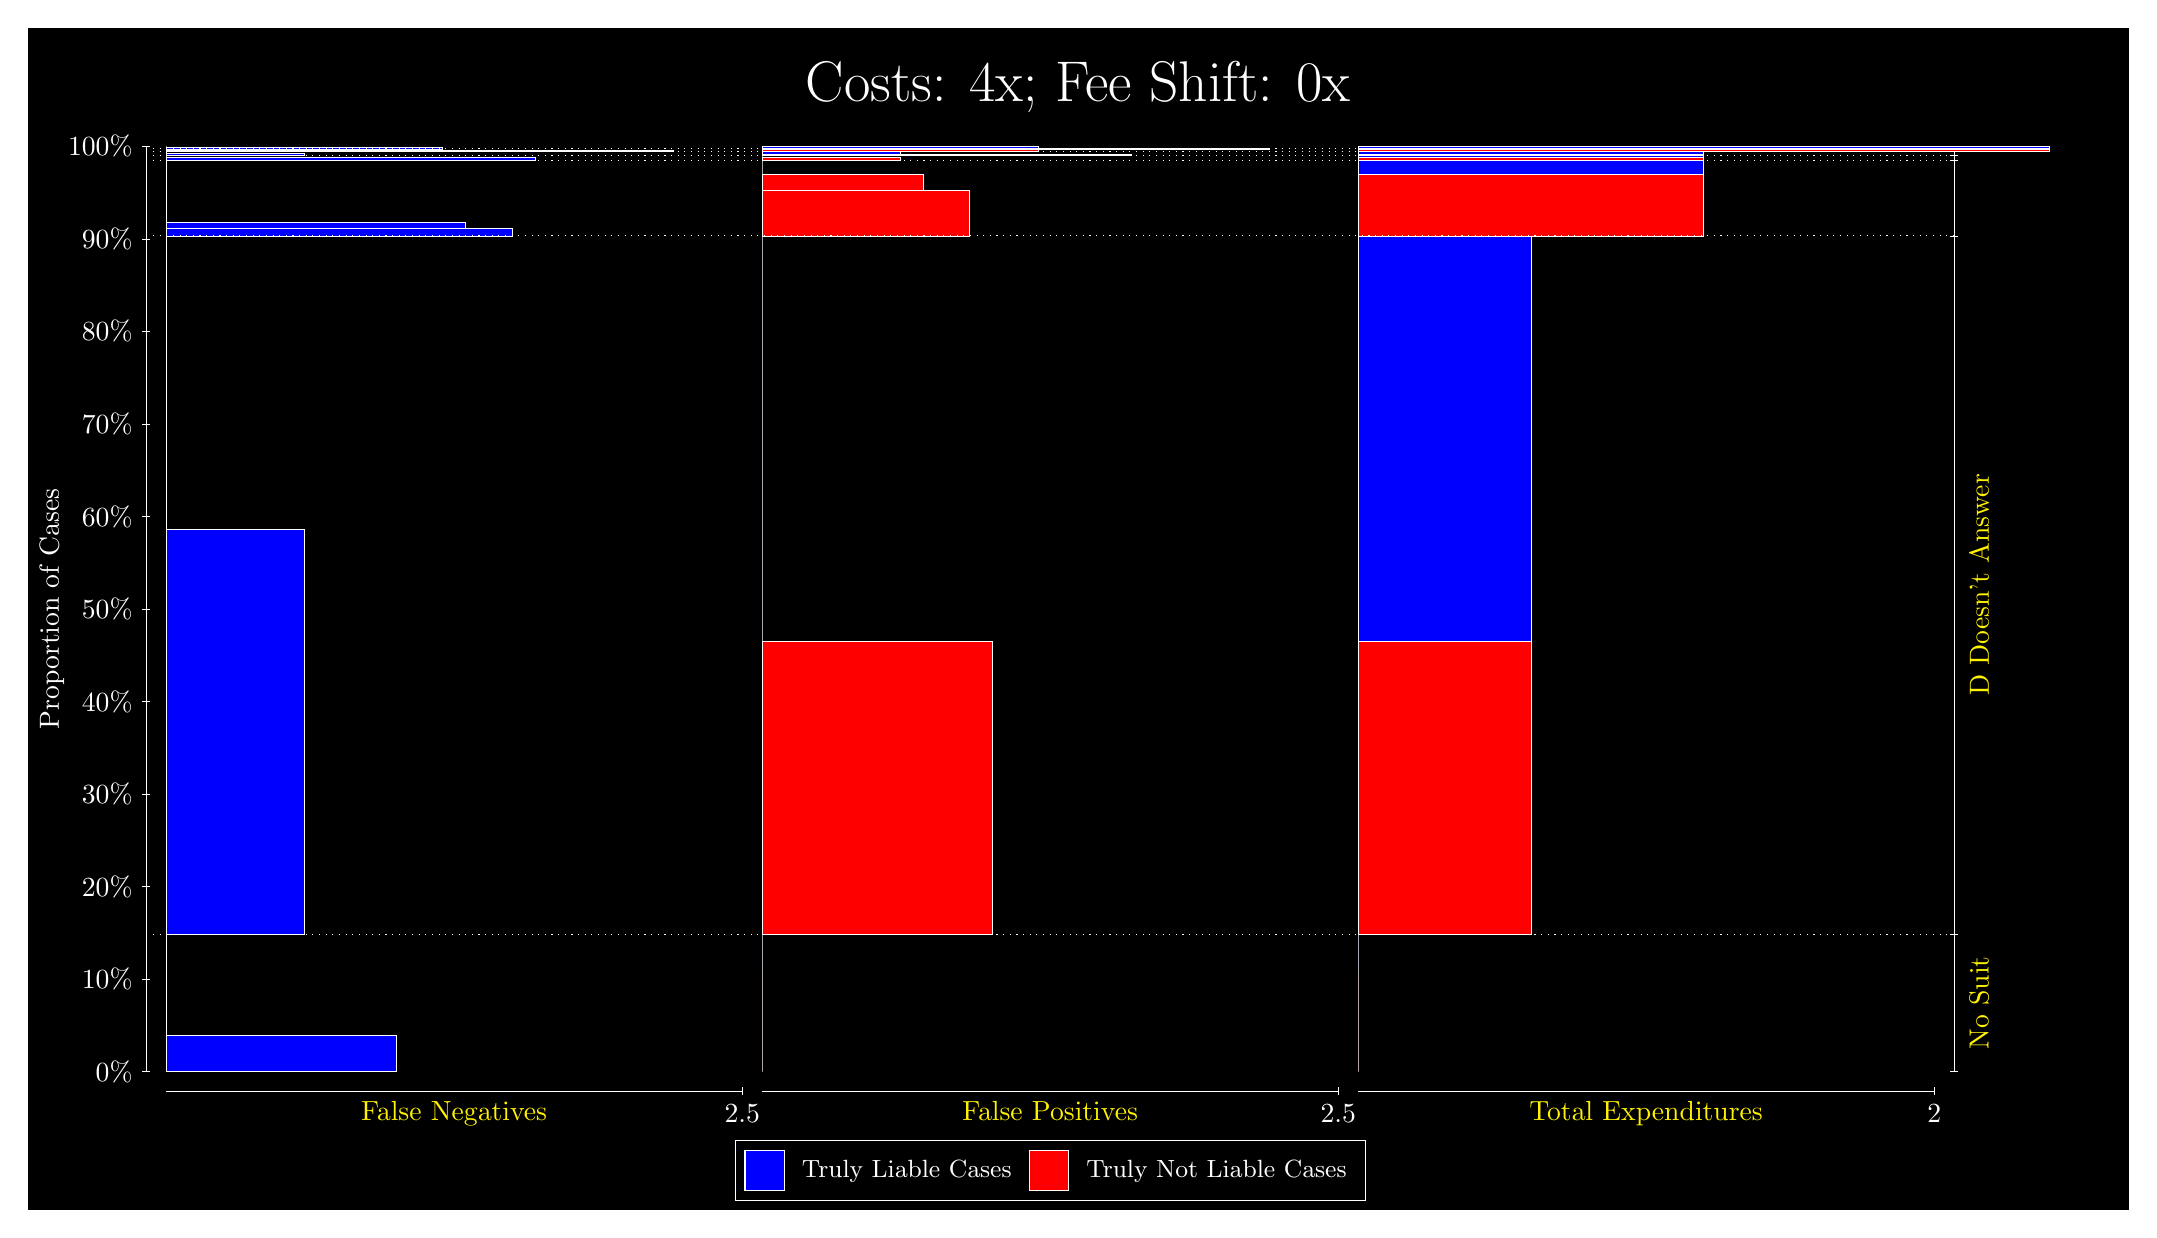
\begin{tikzpicture}
\draw[fill=black] (0,0) rectangle (26.667,15);
\draw[text=white] (0,13.5) rectangle (26.667,15) node[midway] {\huge Costs: 4x; Fee Shift: 0x};
\draw[white, very thin] (1.5,1.75) -- (1.5,13.5);
\node[rotate=90, text=white, anchor=center] at (0.3, 7.625) {Proportion of Cases};
\draw[white, very thin] (1.45,1.75) -- (1.55,1.75);
\node[text=white, anchor=east] at (1.45, 1.75) {0\%};
\draw[white, very thin] (1.45,2.925) -- (1.55,2.925);
\node[text=white, anchor=east] at (1.45, 2.925) {10\%};
\draw[white, very thin] (1.45,4.1) -- (1.55,4.1);
\node[text=white, anchor=east] at (1.45, 4.1) {20\%};
\draw[white, very thin] (1.45,5.275) -- (1.55,5.275);
\node[text=white, anchor=east] at (1.45, 5.275) {30\%};
\draw[white, very thin] (1.45,6.45) -- (1.55,6.45);
\node[text=white, anchor=east] at (1.45, 6.45) {40\%};
\draw[white, very thin] (1.45,7.625) -- (1.55,7.625);
\node[text=white, anchor=east] at (1.45, 7.625) {50\%};
\draw[white, very thin] (1.45,8.8) -- (1.55,8.8);
\node[text=white, anchor=east] at (1.45, 8.8) {60\%};
\draw[white, very thin] (1.45,9.975) -- (1.55,9.975);
\node[text=white, anchor=east] at (1.45, 9.975) {70\%};
\draw[white, very thin] (1.45,11.15) -- (1.55,11.15);
\node[text=white, anchor=east] at (1.45, 11.15) {80\%};
\draw[white, very thin] (1.45,12.325) -- (1.55,12.325);
\node[text=white, anchor=east] at (1.45, 12.325) {90\%};
\draw[white, very thin] (1.45,13.5) -- (1.55,13.5);
\node[text=white, anchor=east] at (1.45, 13.5) {100\%};

\draw[white, very thin] (24.457,1.75) -- (24.457,13.5);
\draw[white, very thin] (24.407,1.75) -- (24.507,1.75);
\node[anchor=west] at (24.407, 1.75) {};
\draw[white, very thin] (24.407,3.4954) -- (24.507,3.4954);
\node[anchor=west] at (24.407, 3.4954) {};
\draw[white, very thin] (24.407,12.362) -- (24.507,12.362);
\node[anchor=west] at (24.407, 12.362) {};
\draw[white, very thin] (24.407,13.325) -- (24.507,13.325);
\node[anchor=west] at (24.407, 13.325) {};
\draw[white, very thin] (24.407,13.385) -- (24.507,13.385);
\node[anchor=west] at (24.407, 13.385) {};
\draw[white, very thin] (24.407,13.437) -- (24.507,13.437);
\node[anchor=west] at (24.407, 13.437) {};
\draw[white, very thin] (24.407,13.467) -- (24.507,13.467);
\node[anchor=west] at (24.407, 13.467) {};
\draw[white, very thin] (24.407,13.5) -- (24.507,13.5);
\node[anchor=west] at (24.407, 13.5) {};

\draw[white, very thin, fill=blue] (1.75,1.75) rectangle (4.6775,2.2052);
\draw[white, very thin, fill=red] (1.75,2.2052) rectangle (1.75,3.4954);
\draw[white, very thin, fill=blue] (1.75,3.4954) rectangle (3.5065,8.6405);
\draw[white, very thin, fill=red] (1.75,8.6405) rectangle (1.75,12.362);
\draw[white, very thin, fill=blue] (1.75,12.362) rectangle (6.1413,12.46);
\draw[white, very thin, fill=blue] (1.75,12.46) rectangle (5.5558,12.54);
\draw[white, very thin, fill=red] (1.75,12.54) rectangle (1.75,13.325);
\draw[white, very thin, fill=blue] (1.75,13.325) rectangle (6.4341,13.355);
\draw[white, very thin, fill=red] (1.75,13.355) rectangle (1.75,13.385);
\draw[white, very thin, fill=blue] (1.75,13.385) rectangle (3.5065,13.418);
\draw[white, very thin, fill=red] (1.75,13.418) rectangle (1.75,13.437);
\draw[white, very thin, fill=blue] (1.75,13.437) rectangle (8.1906,13.447);
\draw[white, very thin, fill=red] (1.75,13.447) rectangle (1.75,13.467);
\draw[white, very thin, fill=blue] (1.75,13.467) rectangle (5.2631,13.49);
\draw[white, very thin, fill=red] (1.75,13.49) rectangle (1.75,13.5);
\draw[white, very thin, fill=red] (9.3189,1.75) rectangle (9.3189,3.0402);
\draw[white, very thin, fill=blue] (9.3189,3.0402) rectangle (9.3189,3.4954);
\draw[white, very thin, fill=red] (9.3189,3.4954) rectangle (12.246,7.217);
\draw[white, very thin, fill=blue] (9.3189,7.217) rectangle (9.3189,12.362);
\draw[white, very thin, fill=red] (9.3189,12.362) rectangle (11.954,12.945);
\draw[white, very thin, fill=red] (9.3189,12.945) rectangle (11.368,13.147);
\draw[white, very thin, fill=blue] (9.3189,13.147) rectangle (9.3189,13.325);
\draw[white, very thin, fill=red] (9.3189,13.325) rectangle (11.075,13.355);
\draw[white, very thin, fill=blue] (9.3189,13.355) rectangle (9.3189,13.385);
\draw[white, very thin, fill=red] (9.3189,13.385) rectangle (14.003,13.403);
\draw[white, very thin, fill=blue] (9.3189,13.403) rectangle (11.075,13.437);
\draw[white, very thin, fill=red] (9.3189,13.437) rectangle (12.832,13.457);
\draw[white, very thin, fill=blue] (9.3189,13.457) rectangle (9.9044,13.467);
\draw[white, very thin, fill=red] (9.3189,13.467) rectangle (15.759,13.477);
\draw[white, very thin, fill=blue] (9.3189,13.477) rectangle (12.832,13.5);
\draw[white, very thin, fill=red] (16.888,1.75) rectangle (16.888,3.0402);
\draw[white, very thin, fill=blue] (16.888,3.0402) rectangle (16.888,3.4954);
\draw[white, very thin, fill=red] (16.888,3.4954) rectangle (19.083,7.217);
\draw[white, very thin, fill=blue] (16.888,7.217) rectangle (19.083,12.362);
\draw[white, very thin, fill=red] (16.888,12.362) rectangle (21.279,13.147);
\draw[white, very thin, fill=blue] (16.888,13.147) rectangle (21.279,13.325);
\draw[white, very thin, fill=red] (16.888,13.325) rectangle (21.279,13.355);
\draw[white, very thin, fill=blue] (16.888,13.355) rectangle (21.279,13.385);
\draw[white, very thin, fill=red] (16.888,13.385) rectangle (21.279,13.403);
\draw[white, very thin, fill=blue] (16.888,13.403) rectangle (21.279,13.437);
\draw[white, very thin, fill=red] (16.888,13.437) rectangle (25.67,13.457);
\draw[white, very thin, fill=blue] (16.888,13.457) rectangle (25.67,13.467);
\draw[white, very thin, fill=red] (16.888,13.467) rectangle (25.67,13.477);
\draw[white, very thin, fill=blue] (16.888,13.477) rectangle (25.67,13.5);
\draw[white, dotted] (1.5,3.4954) -- (24.457,3.4954);
\draw[white, dotted] (1.5,12.362) -- (24.457,12.362);
\draw[white, dotted] (1.5,13.325) -- (24.457,13.325);
\draw[white, dotted] (1.5,13.385) -- (24.457,13.385);
\draw[white, dotted] (1.5,13.437) -- (24.457,13.437);
\draw[white, dotted] (1.5,13.467) -- (24.457,13.467);
\draw[white, very thin] (1.75,1.5) -- (9.0689,1.5);
\node[text=yellow, anchor=north] at (5.4094, 1.5) {False Negatives};
\draw[white, very thin] (9.0689,1.45) -- (9.0689,1.55);
\node[text=white, anchor=north] at (9.0689, 1.45) {2.5};

\draw[white, very thin] (9.3189,1.5) -- (16.638,1.5);
\node[text=yellow, anchor=north] at (12.978, 1.5) {False Positives};
\draw[white, very thin] (16.638,1.45) -- (16.638,1.55);
\node[text=white, anchor=north] at (16.638, 1.45) {2.5};

\draw[white, very thin] (16.888,1.5) -- (24.207,1.5);
\node[text=yellow, anchor=north] at (20.547, 1.5) {Total Expenditures};
\draw[white, very thin] (24.207,1.45) -- (24.207,1.55);
\node[text=white, anchor=north] at (24.207, 1.45) {2};

\node[text=yellow, centered, rotate=90] at (24.777, 2.6227) {No Suit};
\node[text=yellow, centered, rotate=90] at (24.777, 7.9287) {D Doesn't Answer};






\draw (12.978300999999998,1.5) node[draw=none] (baseCoordinate) {};
\begin{scope}[align=center]
        \matrix[scale=0.5, draw=white, below=0.5cm of baseCoordinate, nodes={draw}, column sep=0.1cm]{
            \node[rectangle, draw, minimum width=0.5cm, minimum height=0.5cm, fill=blue] {}; &
            \node[draw=none, font=\small, text=white] (B) {Truly Liable Cases}; &
            \node[rectangle, draw, minimum width=0.5cm, minimum height=0.5cm, fill=red] {}; &
            \node[draw=none, font=\small, text=white] (B) {Truly Not Liable Cases}; \\
            };
\end{scope}

\end{tikzpicture}
\end{document}